Vorweg will ich kurz erklären, was es mit den Tools zur Versionskontrolle auf sich hat.\\
\ \\
Es geht immer darum, eine lokale Kopie der Quellen von einem Server zu laden. Im einfachsten Fall bei Github als ZIP-Datei. Dies ist in den meisten Fälle ausreichend. Der Link ist jedoch für unsere Versionskontrolle interessant. Dort liegt nun das Repository die ich nenne sie jetzt mal Masterkopie. \\
\begin{minipage}[t]{\textwidth}
  \centering
  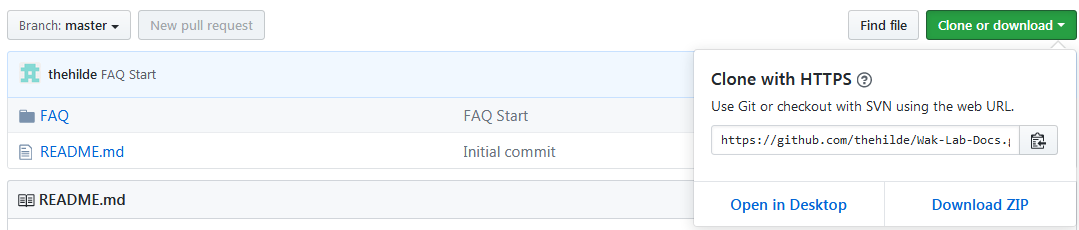
\includegraphics[width=\textwidth]{pictures/Clone.png}
  \captionof{figure}{Eine lokale Kopie Clonen}
  \label{img:Clone}
\end{minipage}
\ \\
Spannend wird es jedoch, wenn die Quellen sich auf dem Server weiterentwickeln oder man sogar selbst eine Verbesserung einbringen will. Die Tools GIT oder SVN managen nun die Synchronisation mit dem Server. Es kann der zeitliche Verlauf der Änderungen angezeigt und zu beliebigen Punkten zurück gesprungen werden. Nie wieder ein "Gestern ging es noch bevor das umgestrickt habe <aarg!>". Welche Änderungen habe ich vor 3 Jahren für XY rein gehackt? Und vor allem Warum? Welchen Fehler wollte ich beseitigen, welches Ticket habe ich bearbeitet? Oder war es der Kollege?  \\
Tools wie Tortoise SVN besitzen eine Explorer Integration, arbeiten über das Kontextmenü und zeigen alle Änderungen automatisch an. \\
\begin{minipage}[t]{\textwidth}
  \centering
  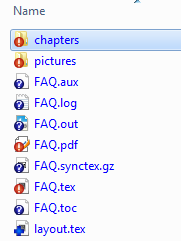
\includegraphics[height=3cm]{pictures/TortoiseSVNChanges.png}
  \captionof{figure}{Tortoise SVN Explorer Integration}
  \label{img:TortoiseSVNChanges}
\end{minipage}
\ \\
Finden Änderungen in der selben Datei aber in unterschiedlichen Bereichen statt, kann das Tool die Änderungen automatisch zusammenführen. In manchen Fällen muss dies jedoch händisch erfolgen.\\
\ \\
Es soll noch gesagt sein, das GIT und SVN zwei verschiedene Tools sind, die etwas abweichende Philosophien haben. Zum Glück sind die beiden auf Github gut verheiratet worden.\\
\ \\
Folgende Dateitypen sind Textbasiert und können prima verwaltet werden.
\begin{itemize}
\item Arduino .ino Dateien
\item Quelltexte z.B. .c .cpp .h .pas .vhdl
\item Natürlich .html .php
\item Windows .ini Dateien
\item Eagle Layout Dateien und Bibliotheken ab Version 6
\item STM Cube32 Dateien
\item \LaTeX .tex Dateien
\item Auch Word ist Prima integriert in Tortoise SVN und öffnet den Word eigenen DIF Viewer.
\end{itemize}


\subsection{Ein Git Beispiel}
Nach dem Login in Github können wir ein neues Projekt erstellen. (Abb. \ref{img:GithubNew})\\
\ \\
\begin{minipage}[t]{\textwidth}
  \centering
  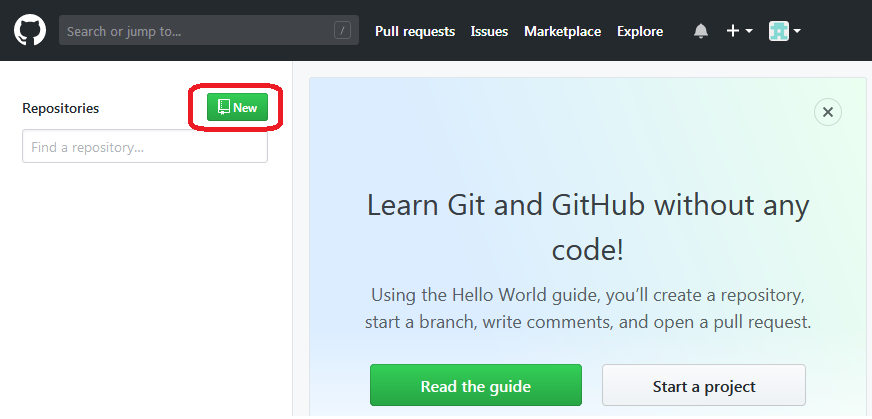
\includegraphics[height=5cm]{pictures/GithubNew.png}
  \captionof{figure}{Neues Projekt}
  \label{img:GithubNew}
  \end{minipage}
\ \\
Das neue Repository bekommt einen Namen eine kurze Beschreibung. Wir legen es Public an, dann ist es auf Github kostenlos. Alternativ können wir später auch unseren Server benutzen. Wir lassen aus unserer Kurzbeschreibung gleich eine Readme Datei erstellen. Hier können wir Markdown-language verwenden um die Anzeige in github etwas zu formatieren.\\
\ \\
\begin{minipage}[t]{\textwidth}
  \centering
  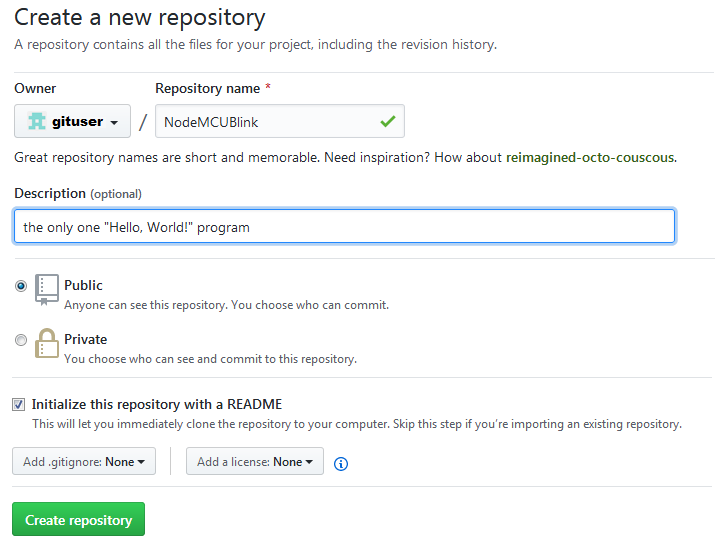
\includegraphics[height=8cm]{pictures/GithubCreate.png}
  \captionof{figure}{Repository erstellen}
  \label{img:GithubCreate}
\end{minipage}
\ \\
Zunächst möchte ich folgende Kurzbeschreibung  nicht vorenthalten \url{https://rogerdudler.github.io/git-guide/index.de.html} dort stehen die wichtigsten git Befehle.\\
Wir legen uns nun lokal ein Verzeichnis an, und clonen uns das Verzeichnis vom Github Server. Den Link findet man im ,,Clone or download`` Menü oben rechts (Abb. \ref{img:Clone}). \\
\begin{verbatim}
C:\Users\SuperDave>md blinky

C:\Users\SuperDave>cd blinky

C:\Users\SuperDave\blinky>git clone https://github.com/thehilde/NodeMCUBlink.git
Cloning into 'NodeMCUBlink'...
remote: Enumerating objects: 3, done.
remote: Counting objects: 100% (3/3), done.
remote: Compressing objects: 100% (2/2), done.
remote: Total 3 (delta 0), reused 0 (delta 0), pack-reused 0
Unpacking objects: 100% (3/3), done.

C:\Users\SuperDave\blinky>dir
 Datenträger in Laufwerk C: ist OS
 Volumeseriennummer: 24F2-3FE3

 Verzeichnis von C:\Users\SuperDave\blinky

30.01.2019  20:22    <DIR>          .
30.01.2019  20:22    <DIR>          ..
30.01.2019  20:22    <DIR>          NodeMCUBlink
               0 Datei(en),              0 Bytes
               3 Verzeichnis(se), 111.597.510.656 Bytes frei

C:\Users\SuperDave\blinky>cd NodeMCUBlink

C:\Users\SuperDave\blinky\NodeMCUBlink>dir
 Datenträger in Laufwerk C: ist OS
 Volumeseriennummer: 24F2-3FE3

 Verzeichnis von C:\Users\SuperDave\blinky\NodeMCUBlink

30.01.2019  20:22    <DIR>          .
30.01.2019  20:22    <DIR>          ..
30.01.2019  20:22                54 README.md
               1 Datei(en),             54 Bytes
               2 Verzeichnis(se), 111.597.510.656 Bytes frei

\end{verbatim}
Die README.md Datei ist gut auf unserem Rechner angekommen. Jetzt Schieben wir weiter Dateien in den Ordner und fügen sie mit ,,add`` dem Projekt hinzu.\\
Am einfachsten ist es erst einmal alle Dateien der Versionsverwaltung hinzuzufügen. Obwohl dies mit Sicherheit nicht das eleganteste ist. Da man Log Dateien, Objekt Dateien oder Binärdateien möglicherweise nicht Versionieren möchte. Einfach weil sie beim compilieren sowieso immer wieder neu erzeugt werden.\\
\begin{verbatim}
C:\Users\SuperDave\blinky\NodeMCUBlink>git add *
warning: LF will be replaced by CRLF in .vscode/c_cpp_properties.json.
The file will have its original line endings in your working directory
warning: LF will be replaced by CRLF in platformio.ini.
The file will have its original line endings in your working directory
\end{verbatim}
In dieser Windows Installation habe ich wohl versehentlich angegeben, dass Zeilenumbrüche korrigiert werden. wir machen erst mal weiter.\\
\begin{verbatim}
C:\Users\SuperDave\blinky\NodeMCUBlink>dir
 Datenträger in Laufwerk C: ist OS
 Volumeseriennummer: 24F2-3FE3

 Verzeichnis von C:\Users\SuperDave\blinky\NodeMCUBlink

30.01.2019  20:47    <DIR>          .
30.01.2019  20:47    <DIR>          ..
30.01.2019  20:47    <DIR>          .pioenvs
30.01.2019  10:44             1.624 .travis.yml
30.01.2019  20:47    <DIR>          .vscode
30.01.2019  20:47    <DIR>          include
30.01.2019  20:47    <DIR>          lib
30.01.2019  10:44               449 platformio.ini
30.01.2019  20:22                54 README.md
30.01.2019  20:47    <DIR>          src
30.01.2019  20:47    <DIR>          test
               3 Datei(en),          2.127 Bytes
               8 Verzeichnis(se), 111.564.550.144 Bytes frei
C:\Users\SuperDave\blinky\NodeMCUBlink>
               
\end{verbatim}
Da wir das Verzeihnis .vscode nicht versionieren wollen, schmeißen wir rekursiv (-r) das gesamte Verzeichnis wieder heraus. Die Datei soll allerdings liegen bleiben als (--cached).\\
\begin{verbatim}
C:\Users\SuperDave\blinky\NodeMCUBlink>git rm -r --cached .vscode
\end{verbatim}
jetzt committen wir das ganze in das lokale Repository\\
\begin{verbatim}
C:\Users\SuperDave\blinky\NodeMCUBlink>git commit -m "Ab damit ins lokale Repo."
[master a0e890c] Ab damit ins lokale Repo.
 8 files changed, 342 insertions(+)
 create mode 100644 .pioenvs/do-not-modify-files-here.url
 create mode 100644 .pioenvs/structure.hash
 create mode 100644 .travis.yml
 create mode 100644 include/README
 create mode 100644 lib/README
 create mode 100644 platformio.ini
 create mode 100644 src/main.cpp
 create mode 100644 test/README

C:\Users\SuperDave\blinky\NodeMCUBlink>

\end{verbatim}
Jetzt steckt alles im lokalen Repository und man kann das Spiel mit add rm und commit so lange treiben bist man lokal ein lauffähiges Programm hat was man auf github mit anderen Teilen will. Nach jedem commit  werden alle Änderungen am Programm archiviert und können später auch wieder hergestellt werden. Deder commit sollte mit einer Nachricht versehen werden, was man in dem Moment verändert hat. Das hilft später bei einem Changelog.\\
Ist man also bereit alles auf github hochzuladen verwendet man push.\\
\begin{verbatim}
C:\Users\SuperDave\blinky\NodeMCUBlink>git push origin master
Enumerating objects: 23, done.
Counting objects: 100% (23/23), done.
Delta compression using up to 4 threads
Compressing objects: 100% (17/17), done.
Writing objects: 100% (22/22), 4.12 MiB | 232.00 KiB/s, done.
Total 22 (delta 1), reused 0 (delta 0)
remote: Resolving deltas: 100% (1/1), done.
To https://github.com/thehilde/NodeMCUBlink.git
   08a2401..4d087a8  master -> master

C:\Users\SuperDave\blinky\NodeMCUBlink>
\end{verbatim}
beim Commit erscheint beim ersten mal eine Passwortabfrage.\\
\ \\
\begin{minipage}[t]{\textwidth}
  \centering
  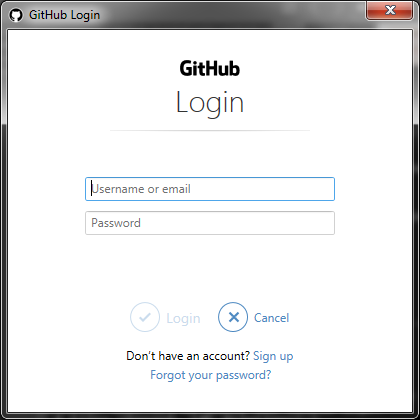
\includegraphics[height=5cm]{pictures/GithubPush.png}
  \captionof{figure}{Passwortabfrage für das hochladen}
  \label{img:GithubPush}
  \end{minipage}
\ \\
Wie man jetzt auf Github sehen kann, ist alles auf Github gelandet, was wir lokal hinzugefügt haben.\\
\ \\
\begin{minipage}[t]{\textwidth}
  \centering
  \includegraphics[height=5cm]{pictures/GithubMaster.png}
  \captionof{figure}{Master Branch auf GitHub}
  \label{img:GithubMaster}
  \end{minipage}  




